\chapter{Memory}

The \procname is connected to the memory through a harvard architecture style interface.
While the interface to the instruction memory is read only, the data memory interface must handle read and write transactions simultaneously.
Externally, both instruction and data memory can be mapped to a Von-Neumann architecture.
The implemented Harvard architecture is more general and allows for two caches to be implemented.

\section{Endianess and Memory Width}
The memory width is defined in the \inlinevhdl{lt16x32\_internal} package.
Currently, memory widths of 32bits are supported only.
Of course, this memory width can be mapped to any other memory width by a memory controller.
The memory organizes data in big endian format.
This can be seen (and changed) in the memory controller, Listing \ref{lst:endianess}.
The same is valid for halfword-accesses.

\begin{vhdl}[Byte-Order in Memory]{lst:endianess}
case byteaddress is
when "00" =>
	dmem_data(7 downto 0) <= word(7 downto 0);
when "01" =>
	dmem_data(7 downto 0) <= word(15 downto 8);
when "10" =>
	dmem_data(7 downto 0) <= word(23 downto 16);
when "11" =>
	dmem_data(7 downto 0) <= word(31 downto 24);
\end{vhdl}

\section{Interface and Timing Description}
\subsection{Instruction Memory Interface}
The \procname is connected to the instruction memory through two ports, as seen in Listing \ref{lst:imem_interface}.
Their datatype definitions can be found in the \inlinevhdl{lt16x32\_global} package.
\begin{vhdl}[Instruction Memory Interface]{lst:imem_interface}
entity core is
port(
	[...]
	-- signals from instruction memory
	in_imem   : in  imem_core;
	-- signals to instruction memory
	out_imem  : out core_imem;
	[...]
);
end entity core;
\end{vhdl}

\subsubsection{Read Access}
As all clocked signals in this design, the address and data signals to the instruction memory must be read on each rising clock edge.
Data must be provided if enable (\inlinevhdl{en}) is asserted and the memory content is read on the next rising clock edge.
This single data rate scheme allows for double data rate memory access to allow for pseudo-simultaneous data and instruction memory access.
A standard signal pattern can found in Figure \ref{fig:signal_imem}.

\begin{figure}[htb]
\centering
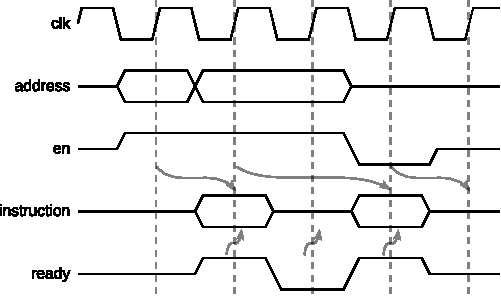
\includegraphics[scale=1]{./figures/signal_imem.pdf}
\caption{Signal Pattern for the Instruction Memory Interface}
\label{fig:signal_imem}
\end{figure}

\subsection{Data Memory Interface}
The \procname is connected to the data memory through two ports, as seen in Listing \ref{lst:dmem_interface}, their datatype definitions can be found in the \inlinevhdl{lt16x32\_global} package.
The data memory interface must be able to handle simultaneous read and write accesses, as these are performed in different pipeline stages and can overlap.
This is good for memory transaction performance but introduces a high memory load.

\begin{vhdl}[Data Memory Interface]{lst:dmem_interface}
entity core is
port(
	[...]
	-- signals from data memory
	in_dmem   : in  dmem_core;
	-- signals to data memory
	out_dmem  : out core_dmem;
	[...]
);
end entity core;
\end{vhdl}

\subsubsection{Read Access}
The read access to the data memory is similar to the instruction memory interface and a standard signal pattern is shown in Figure \ref{fig:signal_imem}.

\subsubsection{Write Access}
In a write access, data and address are supplied at the same time and should be copied to the memory at the rising clock edge if enable is active, see Figure \ref{fig:signal_dmem_write}.
\begin{figure}[htb]
	\centering
	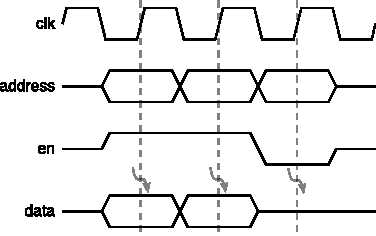
\includegraphics[scale=1]{./figures/signal_dmem_write.pdf}
	\caption{Signal Pattern for Data Memory Write}
	\label{fig:signal_dmem_write}
\end{figure}
\subsection{Memory Bandwidth Solutions}
As mentioned before, the very liberal memory interface demands high memory bandwidth.
In a worst-case scenario three memory accesses are needed per clockcycle (instruction read, data read and data write).

\subsubsection{Instruction Alignment}
Fortunately this worst-case scenario can be avoided by clever instruction alignment.
As standard instructions are 16bit wide and the instruction memory is organized
in 32bit words the instruction memory must be read only once every two clock cycles\footnote{Branching may introduce additional read operations.}.
If memory access instructions are now aligned in such a way, that read/write actions are performed when the instruction memory is idle, a simple single data rate memory is sufficient.
An exemplatory signal pattern is shown in Figure \ref{fig:signal_mem_interlacing}.
Note, that the instruction memory enable must be asserted the whole time,
but the memory controller does not need to read the actual memory,
as the address is changed only every second clock cycle.

\begin{figure}[htb]
	\centering
	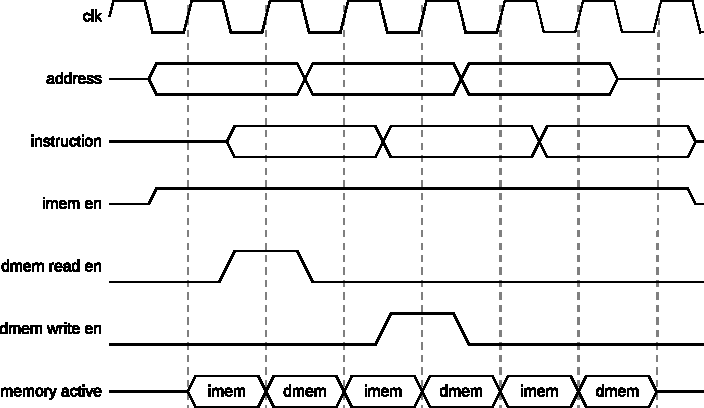
\includegraphics[scale=1]{./figures/signal_mem_interlacing.pdf}
	\caption{Signal Pattern for Memory Interlacing}
	\label{fig:signal_mem_interlacing}
\end{figure}

\subsubsection{Processor Stalling}
If instruction alignment is too cumbersome or the memory is too slow for any other reason, it can deassert the ready signal (\inlinevhdl{ready}) to the processor (per interface).
If \inlinevhdl{ready} is deasserted, the processor is stalled and waits for \inlinevhdl{ready} to become asserted again.

\section{Memory Mapped I/O}
\label{sec:memmappedio}
In the concept of memory mapped input/output (I/O), the processor core does not distinguish between data memory transactions and transactions with other kinds of devices.
Writing to special memory addresses (i.e. outside of the memory range) are forwarded to a device, reading from these addresses means accessing the device's registers.

The systems memory is defined as follows:
\begin{itemize}
\item The instruction memory starts at address zero, its length should be configured to a word boundary.\footnote{The default component uses is configured using a word count.}
\item The data memory starts after the instruction memory, its length is also configurable and should also end on a word boundary.
\item The address space of the peripheral components starts at address \verb=0x000F0000=
\end{itemize}

\section{Memory Controller}
\label{sec:memoryctrl}
A generic memory controller named \verb=dmem= is given.
It has a size of 256 bytes, sectioned in four 64 byte blocks with an access size of one byte.
The default configuration is that its base address is directly after the instruction memory.
It can and should be used to maintain the stack, as frequent accesses to the instruction memory can slow down the performance.
The content of the memory at startup is undefined, and should not be used without initialization.